\chapter{数据库设计}
\section{数据库环境说明}
本系统的数据系统采用PostgreSQL数据库系统。


\section{数据库的命名规则}
\begin{itemize}
	\item 不允许使用缩写
	\item 表名使用单数形式。对于有关联的表,属性名用表名+id的方式来标明这是外表的一个主键
	\item 字段名字不带前缀
\end{itemize}

\section{逻辑设计}

数据模型满足3NF\\
\newpage

\begin{figure}[ht]
	\centering
	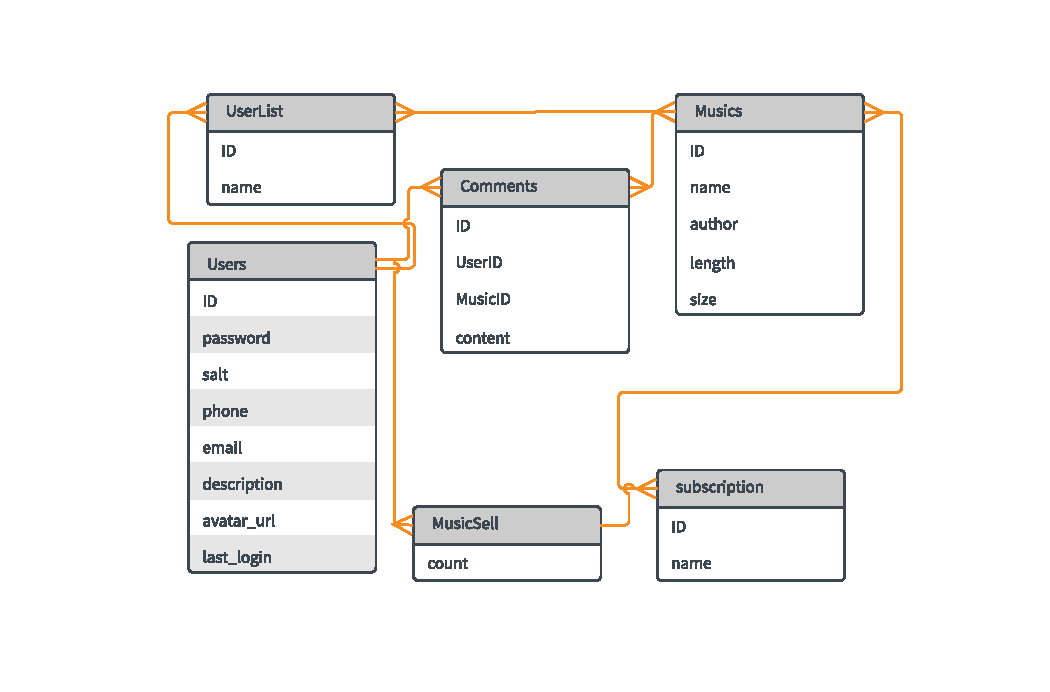
\includegraphics[width=14cm]{database_ER}
	\caption{ER模型图}\label{fig:ER}
\end{figure}

\section{物理设计}

\subsection{数据库产品}

\sout{数据库采用了PostgreSQL,由于暂时数据访问量不大,所以不使用分布式结构。}
\R{数据库采用了PostgreSQL的分布式解决方案PGPool来进行分布式数据存储与查询}

\subsection{实体属性、类型、精度}

\subsubsection{用户数据表设计}

用户数据表保存了用户的基本信息

\begin{table}[htbp]
\centering
\caption{用户数据表Users设计} \label{tab:users-database}
\begin{tabular}{|c|c|c|c|c|}
    \hline
    字段名 & 类型 & 大小 & 说明 & 备注 \\
    \hline
    ID & char & 64 & 用户的唯一标识符 & 主键\\
    \hline
    password & char & 256 & 用户密码的哈希 & · \\
    \hline
    salt & char & 256 & 盐 & · \\
    \hline
    phone & char & 18 & 电话号码 & 外键 \\
    \hline
    email & char & 32 & 电子邮箱 & · \\
    \hline
    description & char & 1024 & 个人自述 & · \\
    \hline
    avatar\_url & char & 256 & 头像地址 & · \\
    \hline
    last\_login & timestamp & 32 & 上次登录时间 & · \\
    \hline
    music\_lists & json & var & 自定义歌单的集合 & . \\
    \hline
\end{tabular}
\note{用户数据表Users设计}
\end{table}

\subsubsection{电话用户对应关系表PhoneToUser设计}

电话用户对应关系表保存了用户电话到用户ID的对应关系

\begin{table}[htbp]
\centering
\caption{电话用户对应关系表PhoneToUser设计} \label{tab:phone-user-database}
\begin{tabular}{|c|c|c|c|c|}
    \hline
    字段名 & 类型 & 大小 & 说明 & 备注 \\
    \hline
    phone & char & 18 & 用户电话号码 & 主键\\
    \hline
    user\_id & char & 64 & 对应用户 & 外键,来自表Users \\
    \hline
\end{tabular}
\note{电话用户对应关系表PhoneToUser设计}
\end{table}

\subsubsection{音乐信息数据库Musics设计}

音乐信息数据库保存了音乐的信息

\begin{table}[htbp]
	\centering
	\caption{音乐信息数据库Musics设计} \label{tab:music-database}
	\begin{tabular}{|c|c|c|c|c|}
		\hline
		字段名 & 类型 & 大小 & 说明 & 备注 \\
		\hline
		ID & char & 64 & 音乐唯一标识符 & 主键\\
		\hline
		name & char & 64 & 音乐名称 & · \\
		\hline
		author & char & 64 & 作者 & · \\
		\hline
		length & smallint & 16 & 时长(秒) & · \\
		\hline
		size & int & 32 & 大小(字节) & · \\
		\hline
	\end{tabular}
	\note{音乐信息数据库Musics设计}
\end{table}

\subsubsection{订阅信息数据库Subscriptions设计}

订阅信息数据库保存了订阅的信息

\begin{table}[htbp]
	\centering
	\caption{订阅信息数据库Subscriptions设计} \label{tab:subscription-database}
	\begin{tabular}{|c|c|c|c|c|}
		\hline
		字段名 & 类型 & 大小 & 说明 & 备注 \\
		\hline
		ID & char & 64 & 订阅唯一标识符 & 主键\\
		\hline
		name & char & 64 & 订阅名称 & · \\
		\hline
		contents & json & var & 包含的音乐的集合  & · \\
		\hline
	\end{tabular}
	\note{订阅信息数据库Subscriptions设计}
\end{table}

\R{
\subsubsection{用户好友关系数据库Friendship设计}
用户好友关系保存了用户之间是否是好友的情况
\begin{table}[htbp]
	\centering
	\R{
	\caption{用户好友关系数据库Friendship设计} \label{tab:friendship-database}
	\begin{tabular}{|c|c|c|c|c|}
		\hline
		字段名 & 类型 & 大小 & 说明 & 备注 \\
		\hline
		user\_ID1 & char & 64 & 用户ID & 主键\\
		\hline
		user\_ID2 & char & 64 & 用户ID & 主键 \\
		\hline
		since & timestamp & 8 & 添加好友的时间  & · \\
		\hline
	\end{tabular}
	\note{用户好友关系数据库Friendship设计}
	}
\end{table}
}


\subsubsection{用户音乐购买信息MusicSells设计}

用户音乐购买信息保存了相当于订阅信息倒排索引的信息

\begin{table}[htbp]
	\centering
	\caption{用户音乐购买信息MusicSells设计} \label{tab:music-sell-database}
	\begin{tabular}{|c|c|c|c|c|}
		\hline
		字段名 & 类型 & 大小 & 说明 & 备注 \\
		\hline
		user\_ID & char & 64 & 用户ID & 主键\\
		\hline
		music\_ID & char & 64 & 音乐ID & 主键 \\
		\hline
		count & smallint & 8 & 累计次数  & · \\
		\hline
	\end{tabular}
	\note{用户音乐购买信息MusicSells设计}
\end{table}

\subsubsection{自定义歌单数据库MusicList设计}

自定义歌单数据库保存了歌单的信息

\begin{table}[htbp]
	\centering
	\caption{自定义歌单数据库MusicList设计} \label{tab:music-list-database}
	\begin{tabular}{|c|c|c|c|c|}
		\hline
		字段名 & 类型 & 大小 & 说明 & 备注 \\
		\hline
		ID & char & 64 & 歌单唯一标识符 & 主键\\
		\hline
		name & char & 64 & 歌单名称 & · \\
		\hline
		contents & json & var & 包含的音乐的集合  & · \\
		\hline
	\end{tabular}
	\note{自定义歌单数据库MusicList设计}
\end{table}

\subsubsection{用户评论Comments设计}

自定义歌单数据库保存了歌单的信息

\begin{table}[htbp]
	\centering
	\caption{用户评论Comments设计} \label{tab:comments-database}
	\begin{tabular}{|c|c|c|c|c|}
		\hline
		字段名 & 类型 & 大小 & 说明 & 备注 \\
		\hline
		ID & char & 64 & 用户评论唯一标识符 & 主键 \\
		\hline
		UserID & char & 64 & 用户ID & 外键 \\
		\hline
		MusicID & char & 64 & 歌曲ID & 外键 \\
		\hline
		comment & char & 512 & 用户对歌曲的评论  & · \\
		\hline
	\end{tabular}
	\note{用户评论Comments设计}
\end{table}

\R{
\subsubsection{用户私人空间状态分享数据库Sharings设计}
用户私人空间状态分享数据库保存了用户在私人空间的分享的情况。
\begin{table}[htbp]
	\centering
	\R{
	\caption{用户私人空间状态分享数据库Sharings设计} \label{tab:sharings-database}
	\begin{tabular}{|c|c|c|c|c|}
			\hline
			字段名 & 类型 & 大小 & 说明 & 备注 \\
			\hline
			share\_ID & char & 64 & 分享ID & 主键 \\
			\hline
			user\_ID & char & 64 & 用户ID & 外键\\
			\hline
			content & JSON & 256 & 用户分享内容 & · \\
			\hline
			when & timestamp & 8 & 用户发送分享时间  & · \\
			\hline
			goods & int32 & 4 & 用户点赞数 & · \\
			\hline
	\end{tabular}
	\note{用户私人空间状态分享数据库Sharings设计}
	}
\end{table}
}

\R{
	\subsubsection{用户私人空间状态分享评论数据库Sharings-Comments设计}
	用户私人空间状态分享数据库保存了用户在私人空间的分享的评论情况。
	\begin{table}[htbp]
		\centering
		\R{
			\caption{用户私人空间状态分享评论数据库Sharings-Comments设计} \label{tab:sharings-comments-database}
			\begin{tabular}{|c|c|c|c|c|}
				\hline
				字段名 & 类型 & 大小 & 说明 & 备注 \\
				\hline
				share\_ID & char & 64 & 分享ID & 主键 \\
				\hline
				user\_ID & char & 64 & 用户ID & 外键\\
				\hline
				content & JSON & 256 & 用户评论内容 & · \\
				\hline
				when & timestamp & 8 & 用户发送评论时间  & · \\
				\hline
			\end{tabular}
			\note{用户私人空间状态分享评论数据库Sharings-Comments设计}
		}
	\end{table}
}

\R{
	\subsubsection{用户私人空间状态分享评论数据库Sharings-Thumbs设计}
	用户私人空间状态分享数据库保存了用户在私人空间的分享的点赞情况。
	\begin{table}[htbp]
		\centering
		\R{
			\caption{用户私人空间状态分享评论数据库Sharings-Thumbs设计} \label{tab:sharings-comments-database}
			\begin{tabular}{|c|c|c|c|c|}
				\hline
				字段名 & 类型 & 大小 & 说明 & 备注 \\
				\hline
				share\_ID & char & 64 & 分享ID & 主键 \\
				\hline
				user\_ID & char & 64 & 用户ID & 外键\\
				\hline
			\end{tabular}
			\note{用户私人空间状态分享评论数据库Sharings-Thumbs设计}
		}
	\end{table}
}

\section{安全性设计}	
通过合理设置权限,只有管理员和应用程序账号
能修改表的数据和读取用户隐私相关的数据。同时,数据库进行定时热备份,保证了数据库
即使在服务器出问题丢失数据的情况下迅速恢复。

\section{数据库管理与维护说明}
监视数据库进程,如果出现无法连接马上告警。

定时更新数据库安全补丁。